% Modern editorial, markup and figure/layout contributions: CC-BY-SA-4.0.
% Historical text and illustrations: Leonhard Euler (1744), public domain.
% Component scope and upstream attribution: see RIGHTS.md.
% Manual vector redraw from E65 Tabula I, Fig. 9.
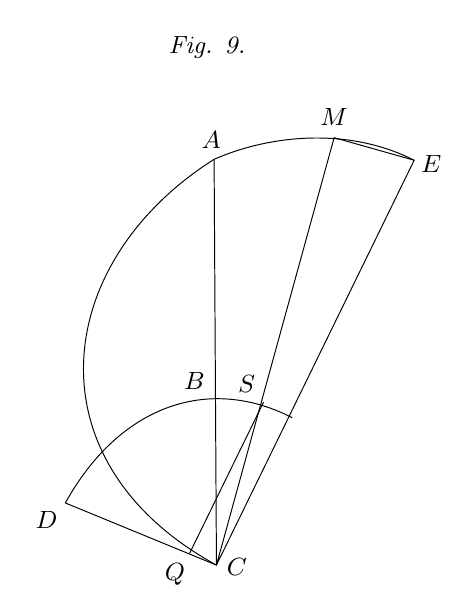
\begin{tikzpicture}[x=1cm,y=1cm,line width=.35pt,font=\small]
\draw (2.8696,0.3886)--(2.8397,5.5418);
\draw (2.8696,0.3886)--(4.3641,5.8168)--(5.3804,5.5299)--(2.8696,0.3886)--(0.9505,1.1777);
\draw (2.5288,0.5380)--(3.4674,2.4571);
\draw (2.8696,0.3886) .. controls (0.4783,1.6978) and (0.7712,4.2326) .. (2.8397,5.5418) .. controls (3.5451,5.8527) and (4.5495,5.9543) .. (5.3804,5.5299);
\draw (0.9505,1.1777) .. controls (1.6500,2.4391) and (2.7918,2.7978) .. (3.8321,2.2598);
\node[anchor=south,inner sep=1pt] at (2.8038,5.6435) {$A$};
\node[anchor=south,inner sep=1pt] at (4.3641,5.9245) {$M$};
\node[anchor=west,inner sep=1pt] at (5.4283,5.4821) {$E$};
\node[anchor=south east,inner sep=1pt] at (2.7620,2.5826) {$B$};
\node[anchor=south east,inner sep=1pt] at (3.4016,2.5348) {$S$};
\node[anchor=north east,inner sep=1pt] at (0.8908,1.1120) {$D$};
\node[anchor=north east,inner sep=1pt] at (2.5109,0.4484) {$Q$};
\node[anchor=west,inner sep=1pt] at (2.9592,0.3707) {$C$};
\node[anchor=south] at (2.7500,6.6957) {\textit{Fig. 9.}};
\end{tikzpicture}
